\documentclass[11pt,letterpaper]{article}
\PassOptionsToPackage{hyphens}{url}
\usepackage[margin=.83in,top=.8in,bottom=.8in,headheight=15pt]{geometry}
\usepackage[T1]{fontenc}
\usepackage{lmodern,amsmath,amssymb,mathtools,bm,booktabs,array,graphicx,tikz}
\usetikzlibrary{arrows.meta,positioning,calc,decorations.pathreplacing,patterns}
\definecolor{ink}{HTML}{17344D}\definecolor{accent}{HTML}{087E8B}\definecolor{pale}{HTML}{EDF5F5}\definecolor{gold}{HTML}{AD6B19}
\providecommand{\dd}{\,\mathrm{d}}\providecommand{\R}{\mathbb{R}}
\providecommand{\E}{\mathbb{E}}\providecommand{\Var}{\operatorname{Var}}
\providecommand{\Cov}{\operatorname{Cov}}\providecommand{\diag}{\operatorname{diag}}
\providecommand{\norm}[1]{\left\lVert#1\right\rVert}
\providecommand{\abs}[1]{\left|#1\right|}
\usepackage{microtype,hyperref,fancyhdr,enumitem,amsthm,sectsty,needspace}
\allsectionsfont{\raggedright}
\hypersetup{colorlinks=true,linkcolor=ink,urlcolor=accent,pdfauthor={Zan Ahmad},pdftitle={Repeated observations, group leakage and predictive baselines / Lecture notes}}
\setlength{\parindent}{0pt}\setlength{\parskip}{6pt}\linespread{1.07}
\setlist{itemsep=3pt,topsep=4pt,leftmargin=*}
\emergencystretch=2em\clubpenalty=10000\widowpenalty=10000
\pagestyle{fancy}\fancyhf{}\fancyhead[L]{\small Computational Cardiology}\fancyhead[R]{\small Lecture 15}
\fancyfoot[L]{\footnotesize Zan Ahmad}\fancyfoot[R]{\footnotesize\thepage}\renewcommand{\headrulewidth}{.3pt}
\newtheorem{proposition}{Proposition}\newtheorem{theorem}{Theorem}\newtheorem{lemma}{Lemma}
\theoremstyle{definition}\newtheorem{definition}{Definition}\newtheorem{example}{Example}
\numberwithin{equation}{section}
\begin{document}
{\small\scshape Computational Cardiology\hfill Lecture 15}\par\medskip
{\raggedright\hyphenpenalty=10000\exhyphenpenalty=10000\LARGE\bfseries\color{ink} Repeated observations, group leakage and predictive baselines\par}\medskip
{\small Lecture notes}\par\bigskip
An evaluation protocol determines which statistical prediction problem is being measured. Repeated observations from one subject are not independent new subjects. A synthetic fingerprint model makes this distinction explicit and permits a controlled comparison of population prediction with recognition of previously observed groups.

\section{Prediction for a new group}
\hypertarget{note-prediction-for-a-new-group}{}\label{note:prediction-for-a-new-group}
{\small \href{slides.html\#frame=repeated-rows-share-a-latent-group\&step=1}{Slides for this section}}\par
A predictive task is incomplete until we say who or what the model will encounter. Predicting an outcome for an entirely new person differs from predicting another observation of someone already represented in training. The same table can support either question, but its evaluation must match the intended use. Our core question is transfer to previously unseen groups. A group stands for a synthetic subject with repeated measurements; it is not a real patient. There is one stable binary outcome per group and no clinical endpoint being modeled.

The companion creates 120 groups with four observations each. One feature contains a weak population-level signal about the group outcome. Eight other features are stable random fingerprints, drawn independently of the outcome, with small observation noise. A fingerprint can help recognize a known group even though it does not predict the outcome of a newly generated group. This deliberately exaggerated construction makes the failure mechanism visible. It does not claim that any particular medical dataset has this exact structure.

Before fitting, write down when each feature would be available and whether the outcome is already known. In an actual longitudinal problem, an apparently useful feature measured after the prediction time can invalidate the experiment even if group IDs are disjoint. Our synthetic rows have no time-to-event meaning; the four observation numbers organize the split without representing disease progression.

A useful schematic model is $x_{gr}=s(y_g)+a_g+\epsilon_{gr}$, where $g$ identifies a group and $r$ a repeat. The shared fingerprint $a_g$ induces dependence between rows from one group even if it is independent of the outcome $y_g$ across groups. Knowing another labeled row from group $g$ can therefore help identify its label without learning a population relation.
\section{Row disjointness and group disjointness}
\hypertarget{note-row-disjointness-and-group-disjointness}{}\label{note:row-disjointness-and-group-disjointness}
{\small \href{slides.html\#frame=the-new-group-condition-panel-1\&step=1}{Slides for this section}}\par
The valid protocol trains on the first three observations of 80 groups and tests on the fourth observation of 40 other groups. Thus 240 training rows and 40 test rows have no group overlap. The controlled contaminated protocol keeps exactly those 40 test rows but replaces 40 training groups with the test groups, using their first three observations. It still has 240 training rows from 80 groups. Matching row counts and test cases helps isolate group membership as the main design difference, although the training identities necessarily change.

Both protocols pass a row-index disjointness test: the exact test observations were never training rows. Only the proper protocol passes a group-disjointness test. The audit function raises an error for shared group IDs when the unseen-group requirement is enabled. We disable that requirement explicitly only inside the labeled counterexample branch. Group-aware cross-validation extends the same principle to repeated folds; the scikit-learn grouped-data section explains that each validation fold must contain groups absent from its training fold.

The forty test groups are balanced by design for this demonstration, with twenty outcomes of each class. That is a sampling choice, not an estimated population prevalence. A real protocol also needs to consider sites, acquisition devices, calendar time and repeated samples. Holding out people does not automatically establish transfer to a different hospital or future period.

Let $G_{train}$ and $G_{test}$ be the sets of group identifiers. New-group evaluation requires
\[
 G_{train}\cap G_{test}=\varnothing,
\]
which is stronger than disjoint row indices. In the contaminated counterexample, rows remain distinct but group labels can be transferred through nearby fingerprints. Holding the same forty test rows fixed makes this change in available information visible.
\begin{center}\begin{minipage}{.98\linewidth}\centering
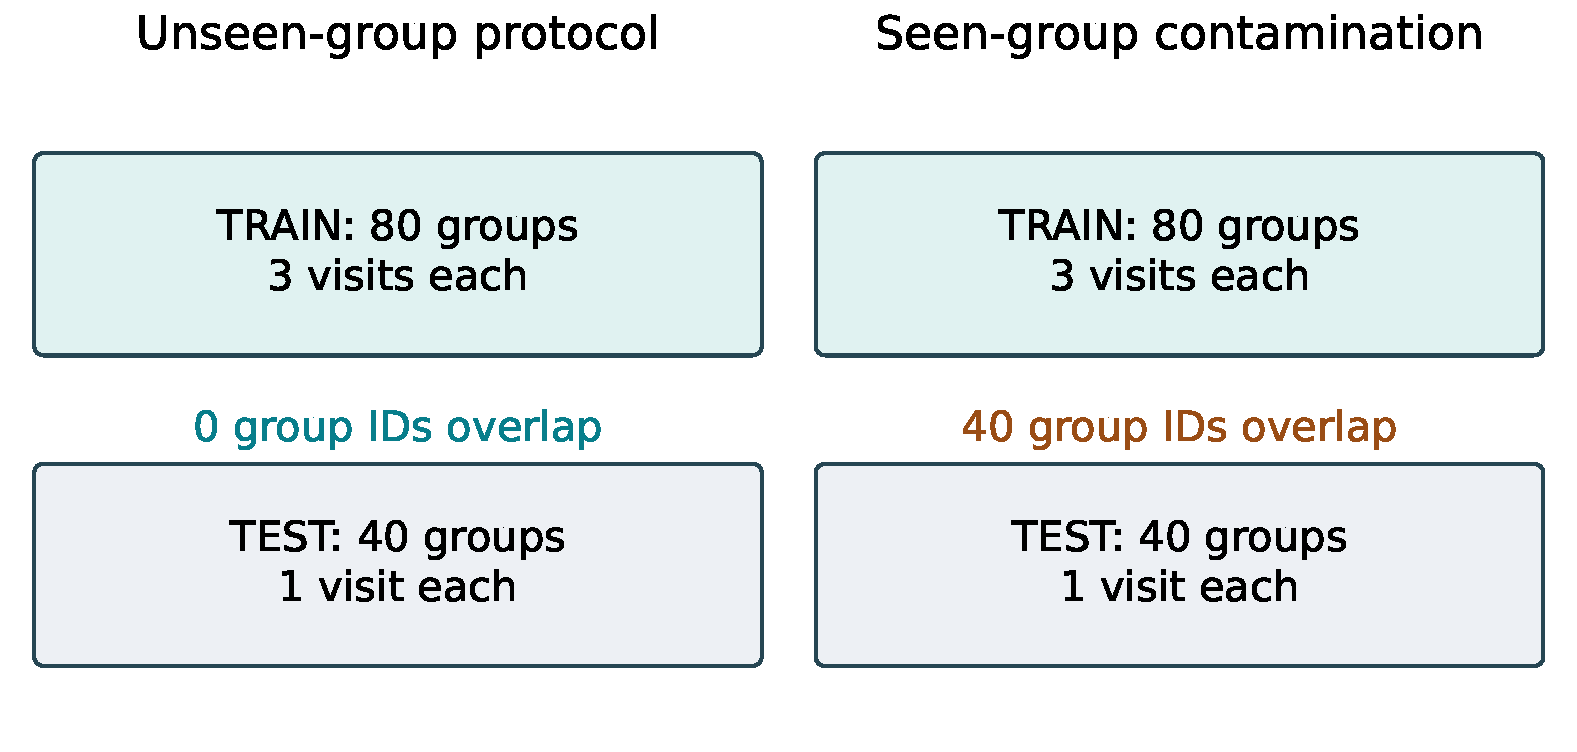
\includegraphics[width=.96\linewidth,height=.57\textheight,keepaspectratio]{group-protocol.pdf}\par\smallskip
{\small Both protocols use 240 training rows from 80 groups and the identical 40 final-observation test rows. Shared group counts are zero versus forty. The contaminated protocol uses other observations of the test groups.}
\end{minipage}\end{center}
\section{Constant, logistic and nearest-neighbor baselines}
\hypertarget{note-constant-logistic-and-nearest-neighbor-baselines}{}\label{note:constant-logistic-and-nearest-neighbor-baselines}
{\small \href{slides.html\#frame=the-constant-baseline\&step=1}{Slides for this section}}\par
The constant classifier uses the training class proportion and predicts class zero on a tie. It establishes what a model can achieve without using features. The signal-only logistic model uses the first feature, a fitted slope and an intercept. Its score is a sigmoid of a linear expression; a threshold of 0.5 gives the predicted class. We use a small fixed squared-slope penalty and do not search for a favorable setting on the test cases. This baseline asks whether the declared population signal supports prediction.

The one-nearest-neighbor baseline uses all nine standardized features and copies the label of the closest training row. Standardization makes each feature's training variation comparable in the distance. It is not a biological weighting scheme. Near-duplicate fingerprints from the same group are extremely close, so this model exposes the advantage of recognizing an already-seen group. Under the proper split, every candidate neighbor belongs to someone else. A more flexible model is not automatically a better test of the intended generalization question.

\[
\widetilde{x}_j=\frac{x_j-\mu_j^{\mathrm{train}}}{s_j^{\mathrm{train}}},\qquad p=\frac{1}{1+e^{-(w\widetilde{x}_1+b)}}
\]
Features are dimensionless synthetic measurements. Means and standard deviations are learned only from the current training subset; a constant feature uses scale one.

For the signal-only model, with $z_i=w\widetilde x_{i1}+b$, the penalized objective is
\[
 J(w,b)=\frac1N\sum_i[\log(1+e^{z_i})-y_i z_i]+\frac\lambda2w^2.
\]
Its derivatives are $\partial_wJ=N^{-1}\sum_i(p_i-y_i)\widetilde x_{i1}+\lambda w$ and $\partial_bJ=N^{-1}\sum_i(p_i-y_i)$. The nearest-neighbor rule instead selects $j_* =\arg\min_{j\in train}\|\widetilde x-\widetilde x_j\|^2$ and returns $y_{j_*}$. These baselines use different information and different inductive assumptions.
\section{Training-dependent transformations}
\hypertarget{note-training-dependent-transformations}{}\label{note:training-dependent-transformations}
{\small \href{slides.html\#frame=fit-the-coordinate-transformation-on-training-data\&step=1}{Slides for this section}}\par
Every fitted transformation is part of the model. Compute feature means and standard deviations from training rows, then reuse them unchanged for test rows. A test-set average is still information from the test set even if no labels are used. The scikit-learn pitfalls documentation makes this fit-versus-transform distinction explicit. A pipeline can help implement it, but the analyst must still choose a valid split and ensure that no forbidden information was encoded earlier in the feature table.

The companion includes an invariance check: add a large offset only to test features and recompute the training scaler. Its fitted means and scales must remain unchanged. Test predictions will generally change, which is expected; training parameters must not. This distinguishes legitimate application of a frozen model from accidental refitting during evaluation. Another check sends a two-point example through nearest-neighbor prediction, verifying the distance calculation without relying on the main synthetic result.

The standardized distance is
\[
 \|\widetilde x-\widetilde x_j\|^2=
 \sum_k\frac{(x_k-x_{jk})^2}{(s_k^{train})^2}.
\]
Thus fitting the scaler also fits the metric used by nearest neighbor. Recomputing scales on test cases would change that metric after seeing the evaluation distribution, even without labels.
\section{Confusion matrices and class-conditional error}
\hypertarget{note-confusion-matrices-and-class-conditional-error}{}\label{note:confusion-matrices-and-class-conditional-error}
{\small \href{slides.html\#frame=read-the-confusion-matrix\&step=1}{Slides for this section}}\par
In the proper split, the constant baseline has accuracy 0.50, signal-only logistic regression 0.725, and all-feature nearest neighbor 0.65. The contaminated nearest-neighbor score becomes 1.00 on the same test cases. This is a successful demonstration of recognition, not evidence of perfect prediction for new people. The signal-only model changes less because it lacks the high-dimensional fingerprint. These values describe one deterministic realization with forty test groups; they are not confidence bounds or estimates of clinical utility.

Accuracy counts all correct classifications equally. Class-specific recall instead divides correctly identified members of one class by the total members of that class. Balanced accuracy averages the two recalls. In our balanced test set it equals ordinary accuracy, but the two can diverge sharply under imbalance. The result file stores confusion matrices with true classes in rows and predicted classes in columns, making the denominators auditable. A missing class should make its recall unavailable rather than silently appear perfect.

Choose a metric based on the scientific error question before examining model rankings. Predictive discrimination also differs from probability calibration. No threshold or accuracy from this synthetic example should be used as a medical decision rule.

\[
\mathrm{BA}=\frac12\left(\frac{TN}{TN+FP}+\frac{TP}{TP+FN}\right)
\]
TN and FP are counts in the true-zero row; TP and FN are counts in the true-one row. Both true classes must be present.

If class prevalence is $\pi=P(Y=1)$, expected accuracy is $(1-\pi)\,\mathrm{TNR}+\pi\,\mathrm{TPR}$. Balanced accuracy replaces these prevalence weights by one half. The two agree on the deliberately balanced test sample, but they represent different summaries in general.
\begin{center}\begin{minipage}{.98\linewidth}\centering
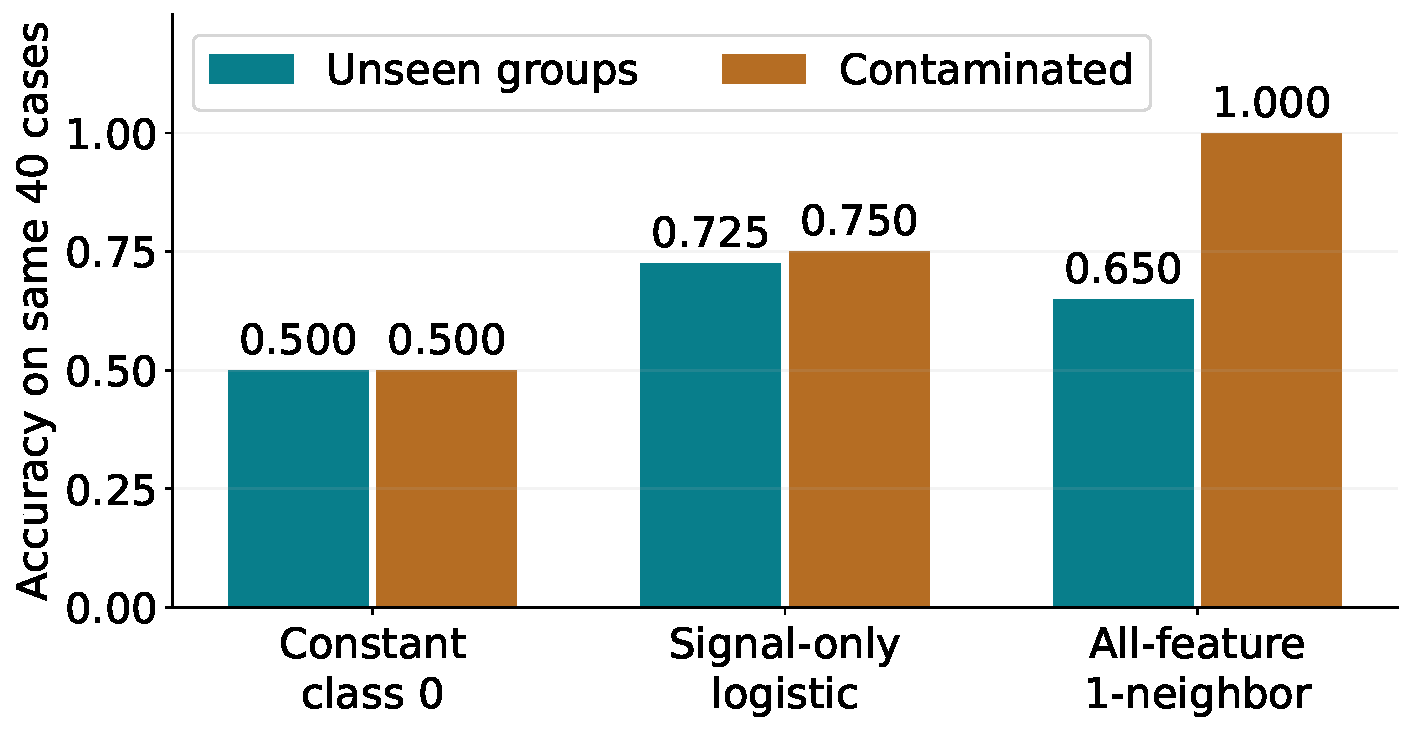
\includegraphics[width=.96\linewidth,height=.57\textheight,keepaspectratio]{baseline-comparison.pdf}\par\smallskip
{\small Accuracy on forty balanced synthetic test groups. The all-feature nearest-neighbor baseline reaches 1.00 only when those groups have other observations in training. This is one controlled realization, without confidence intervals.}
\end{minipage}\end{center}
\section{The scope of the estimated prediction risk}
\hypertarget{note-the-scope-of-the-estimated-prediction-risk}{}\label{note:the-scope-of-the-estimated-prediction-risk}
{\small \href{slides.html\#frame=recognition-is-not-new-group-prediction\&step=1}{Slides for this section}}\par


A held-out group score estimates performance under the chosen group-generating distribution. It does not establish transfer to a new acquisition site, later time or changed feature availability. More repeated rows can improve estimation within a represented group without adding the same amount of information about new groups. The split unit and prediction-time information define the scope of the resulting risk estimate.
\bigskip
\section*{Exercises}
\par\noindent\begin{minipage}{\linewidth}
\subsection*{AC15-E1. Audit repeated observations}
Rows 0--7 have group IDs [A,A,B,B,C,C,D,D]. Training rows are [0,2,4,6] and test rows are [1,3,5,7].

\textbf{a} Compute the number of shared row IDs and shared group IDs.

\end{minipage}\par\medskip
\textbf{b} Construct a split with two whole training groups and two whole test groups.

\textbf{c} Which target is addressed by the original split, and why is it unsuitable for a new-person claim?

\par\noindent\begin{minipage}{\linewidth}
\subsection*{AC15-E2. Choose denominators}
A binary classifier has true-row/predicted-column confusion matrix [[45,5],[8,2]].

\textbf{a} Compute accuracy and class-one recall.

\end{minipage}\par\medskip
\textbf{b} Compute class-zero recall and balanced accuracy.

\textbf{c} Compare with a classifier that always predicts zero. Why can the headline accuracy be misleading?

\par\noindent\begin{minipage}{\linewidth}
\subsection*{AC15-E3. Protect the preprocessing boundary}
A training feature has mean 10 and standard deviation 2. One test feature is 14; a second test feature is later changed from 12 to 1000.

\textbf{a} Standardize the first test feature using the frozen training transform.

\end{minipage}\par\medskip
\textbf{b} Should changing the other test feature alter this value or the fitted scaler? Explain.

\textbf{c} Name two other learned preprocessing operations that require the same protection, and one input-time leak a pipeline alone cannot fix.

\par\noindent\begin{minipage}{\linewidth}
\subsection*{AC15-E4. Draft the evaluation protocol}
The intended use is prediction for a new individual. There are repeated scans, two sites and a candidate outcome measured after the scans.

\textbf{a} State the group rule and feature-availability rule.

\end{minipage}\par\medskip
\textbf{b} Name two transparent baselines and a metric that exposes a failure ordinary accuracy can conceal.

\textbf{c} State a remaining generalization question and how it changes the evaluation.

\section*{References}
\noindent\begin{minipage}{\linewidth}
Zan Ahmad, Advanced Topics in Computational Cardiology syllabus, Fall 2024. PDF pages 1--2.

\end{minipage}\par\medskip
\noindent\begin{minipage}{\linewidth}
scikit-learn, Common pitfalls and recommended practices. Sections 12.1, 12.2 and 12.2.1.

\url{https://scikit-learn.org/stable/common_pitfalls.html}
\end{minipage}\par\medskip
\noindent\begin{minipage}{\linewidth}
scikit-learn, Cross-validation: evaluating estimator performance. Sections 3.1.2.4 and 3.1.2.4.1; introductory train/validation/test discussion.

\url{https://scikit-learn.org/stable/modules/cross_validation.html}
\end{minipage}\par\medskip
\end{document}
